%%%%%%%%%%%%%%%%%%%%%%%%%packages%%%%%%%%%%%%%%%%%%%%%%%%%%%
\documentclass[a4paper,12pt,titlepage]{article}
\usepackage[francais]{babel}
\usepackage[utf8]{inputenc}
\usepackage[pdftex]{graphicx}
\usepackage{vmargin}
\usepackage{fancyhdr}
\usepackage{lastpage}
\usepackage{color}
\usepackage{xcolor}
\definecolor{LightGray}{gray}{0.7}
\usepackage{minted}
\usepackage{titlesec}
\usepackage{circuitikz}
 \usepackage{siunitx}


%%%%%%%%%%%%%%%%%%%%%%%%%%%%%%%%%%%%%%%%%%%%%%%%%%%%%%%%%%%%
\pagestyle{fancy}
\renewcommand{\headrulewidth}{0.2pt}
\renewcommand{\footrulewidth}{0.2pt}

\title{
    
\includegraphics[width=0.15\textwidth]{logos/UM.png}
    \hspace{1cm}    
    
\includegraphics[width=0.4\textwidth]{logos/Polytech.png}\\
    \vspace{5cm}
    \textbf{T.P.\\Électronique}\\ TEYSSIER Maxime\\ \vspace{1cm}Exemple d’utilisation de Pspice : manipulation autour de la diode
    \vfill
}
\begin{document}
\cfoot{Pages \thepage/\pageref{LastPage}}
\lhead{TEYSSIER Maxime}
\rhead{EII Systèmes Embarqués 3}
\rfoot{Polytech' Montpellier}
\lfoot{UM}
\maketitle
\newpage
%%%%%%%%%%%%%%%%%%%%%%%%%%%%%%%%%%%%%%%%%%%%%%%%%%%%%%%%%%%%%%

\begin{center}
    Modèle \fbox{grands signaux}
\end{center}



\begin{minted}[
    baselinestretch=1.4,
    bgcolor=LightGray,
    fontsize=\footnotesize]
{php}
caracteristique directe
* fichier diode.cir
.lib eval.lib
Vdiode 1 0
D 1 0 D1N4002 ; diode de redressement
.DC Vdiode 0 1 1m ; increment de 1 mV
.probe
.end
\end{minted}
\begin{center}
    \textit{Fichier .cir donné en exemple sur le sujet}\\
\end{center}

\begin{center}
    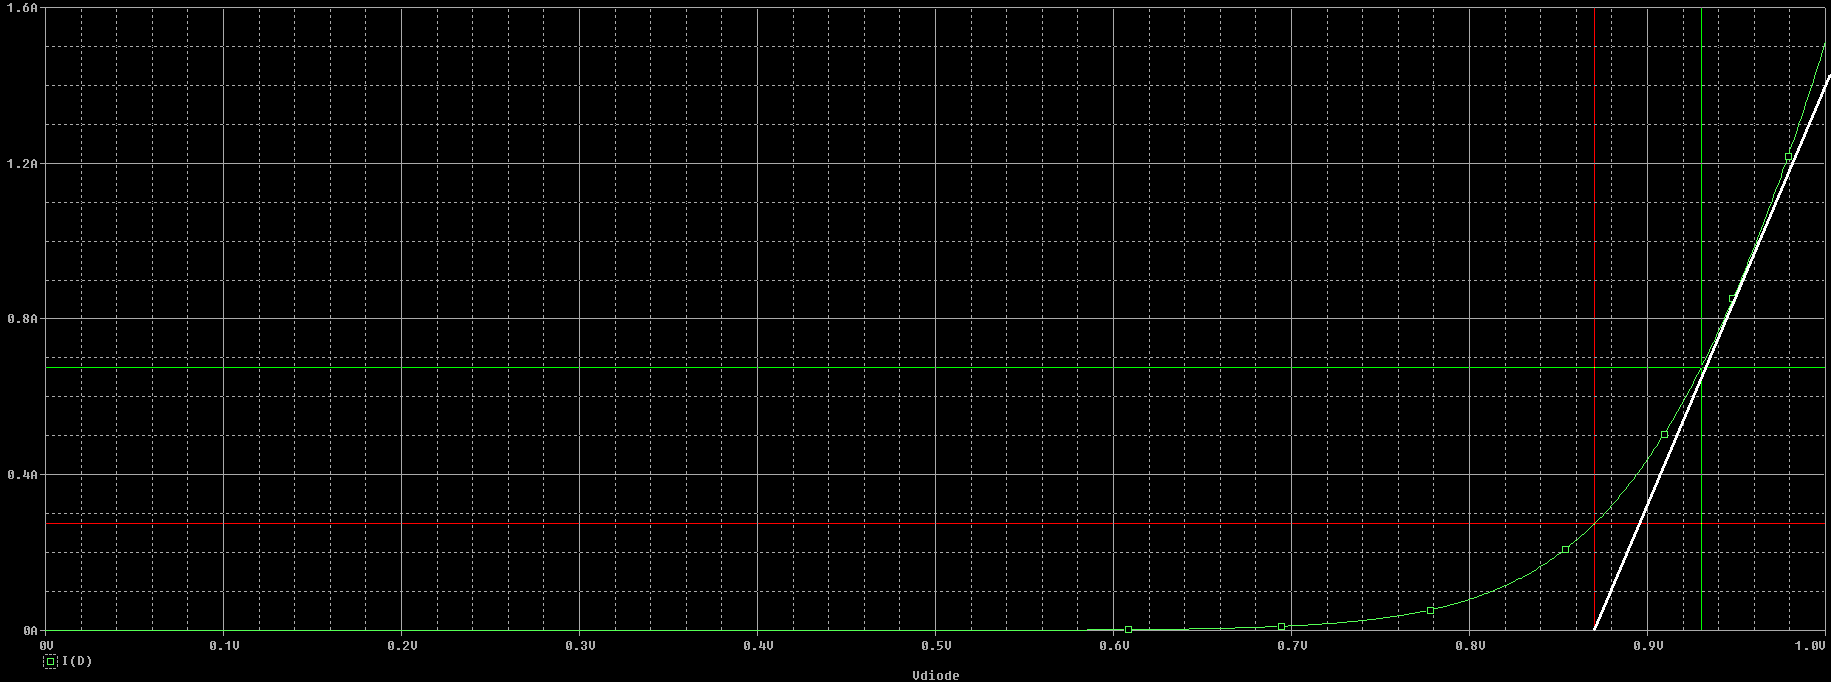
\includegraphics[width=\textwidth]{screenshots/Diode1.png}\\
    \textit{Simulation 1}\\
\end{center}


Les valeurs que j'ai choisis sont: (0.930V,0.701A) et (0.870V,0.216A).\\

\begin{center}
    $R_D=\frac{\Delta V}{\Delta I}=\frac{0.930 - 0.870}{0.701 - 0.216} \approx 0.124 \Omega$ \\ \vspace{2cm}
    
    Modèle \fbox{petits signaux} Statique\\
\end{center}

Les coordonnées de mon point de polarisation sont : (0.900V,0.439A)\\

\begin{center}
    $R_{eq}+R_s = \frac{0.9167 - 0.9165}{0.561 - 0.559} \approx 0.133 \Omega $ \\
\end{center}

Via le fichier \textit{.out} extrait de la simulation, nous savons que $R_s \approx 0.033$. Donc $R_eq = R_s - 0.133 \approx 0.1$. \\


\begin{minted}[
    baselinestretch=1.4,
    bgcolor=LightGray,
    fontsize=\footnotesize]
{php}

Caracteristique directe
* fichier diode.cir
.lib eval.lib
Vdiode 1 0 DC=0.9
D 1 0 D1N4002 ; diode de redressement
.OP
.probe
.end

\end{minted}
\begin{center}
    \textit{Fichier .cir avec la tension de notre point de polarisation}\\
\end{center}


\begin{minted}[
    baselinestretch=1.4,
    bgcolor=LightGray,
    fontsize=\footnotesize]
{php}
 ****     Diode MODEL PARAMETERS
******************************************************************************
               D1N4002         
          IS   14.110000E-09 
           N    1.984        
         ISR  100.000000E-12 
         IKF   94.81         
          BV  100.1          
         IBV   10            
          RS     .03389      
          TT    4.761000E-06 
         CJO   51.170000E-12 
          VJ     .3905       
           M     .2762       

**** 10/06/19 14:33:55 ******* PSpice Lite (March 2016) ******* ID# 10813 ****

\end{minted}
\begin{center}
    \textit{Résultat de la simulation 2 - Verification de $Is$,n et $R_s$}
\end{center}

Nous pouvons remarquer que les valeurs sont bien les mêmes que donné dans le sujet.\\

\begin{minted}[
    baselinestretch=1.4,
    bgcolor=LightGray,
    fontsize=\footnotesize]
{php}
**** DIODES
NAME         D         
MODEL        D1N4002   
ID           4.39E-01 
VD           9.00E-01 
REQ          1.17E-01 
CAP          4.06E-05 
          JOB CONCLUDED

**** 10/06/19 14:33:55 ******* PSpice Lite (March 2016) ******* ID# 10813 ****
\end{minted}

\begin{center}
    \textit{Résultat de la simulation 2 - Affichage de $I_D$,$V_D$ et $R_{eq}$}
\end{center}

Pour calculer la chute de tension au bornes de $R_s$:
$V_{R_S} = R_S \times I_S$\\
\begin{center}
    $V_{R_S} = 0.034 \times 14.11 \times 10^{-9} = 4.797 \times 10^{-10}$V
\end{center}

On peut en déduire la valeur de $V_{PN}$:
\begin{center}
    $V_{PN} = V_D - V_{R_S} = 0.87 - 4.797 \times 10^{10} \approx 0.869$V \\
\end{center}

Pour calculer $V_T$ nous utiliserons la formule $V_T = K\times\frac{T}{q}$\\
\begin{center}
    $V_T= 1,38\times 10^{-23} \times \frac{300}{1,6\times 10^{-19}} = 0.0259$V\\
\end{center}

La relation de Shockley appliquée à la diode intrinsèque nous permet de calculer le courant: \\

\begin{center}
    $I_{D_Intra} = I_S \times (e^{\frac{V}{nV_T}}-1) = 14,11\times10^{-9}\times (e^{\frac{0.9}{1,984\times 0.0259}}-1) = 0,57$A\\
\end{center}

\textbf{Le point de polarisation choisi au début ne me fournit pas la bonne valeur au final.}\\

Nous devons $R_{eq}$ par le calcul:
\begin{center}
    $R_{eq} = \frac{nV_T}{I} = \frac{1.984 \times 0.026}{0.439} = 0.117\Omega$\\
\end{center}
Nous retrouvons bien la valeur affiché par Pspice.\\
\vspace{2cm}    
\begin{center}
    Modèle \fbox{petits signaux} Dynamique\\
\end{center}   

Le choix de d'avoir les valeurs: 1kHz, d'amplitude 5mV et aucun offset permet de ne pas avoir de valeurs négatives et ainsi on outre passe la saturation.\\

\begin{minted}[
    baselinestretch=1.4,
    bgcolor=LightGray,
    fontsize=\footnotesize]
{php}
DM
* DM3
.lib eval.lib
VE 1 0 DC=0.9
Vet 1 2 SIN (0 5m 1k 0 0 0)
D 2 0 D1N4002 ; diode de redressement
.TRAN 5u 5m
.probe
.end
\end{minted}

\begin{center}
    \textit{Fichier .cir  avec utilisation la directive \textit{.TRAN}}\\
    \vspace{1cm}\\
    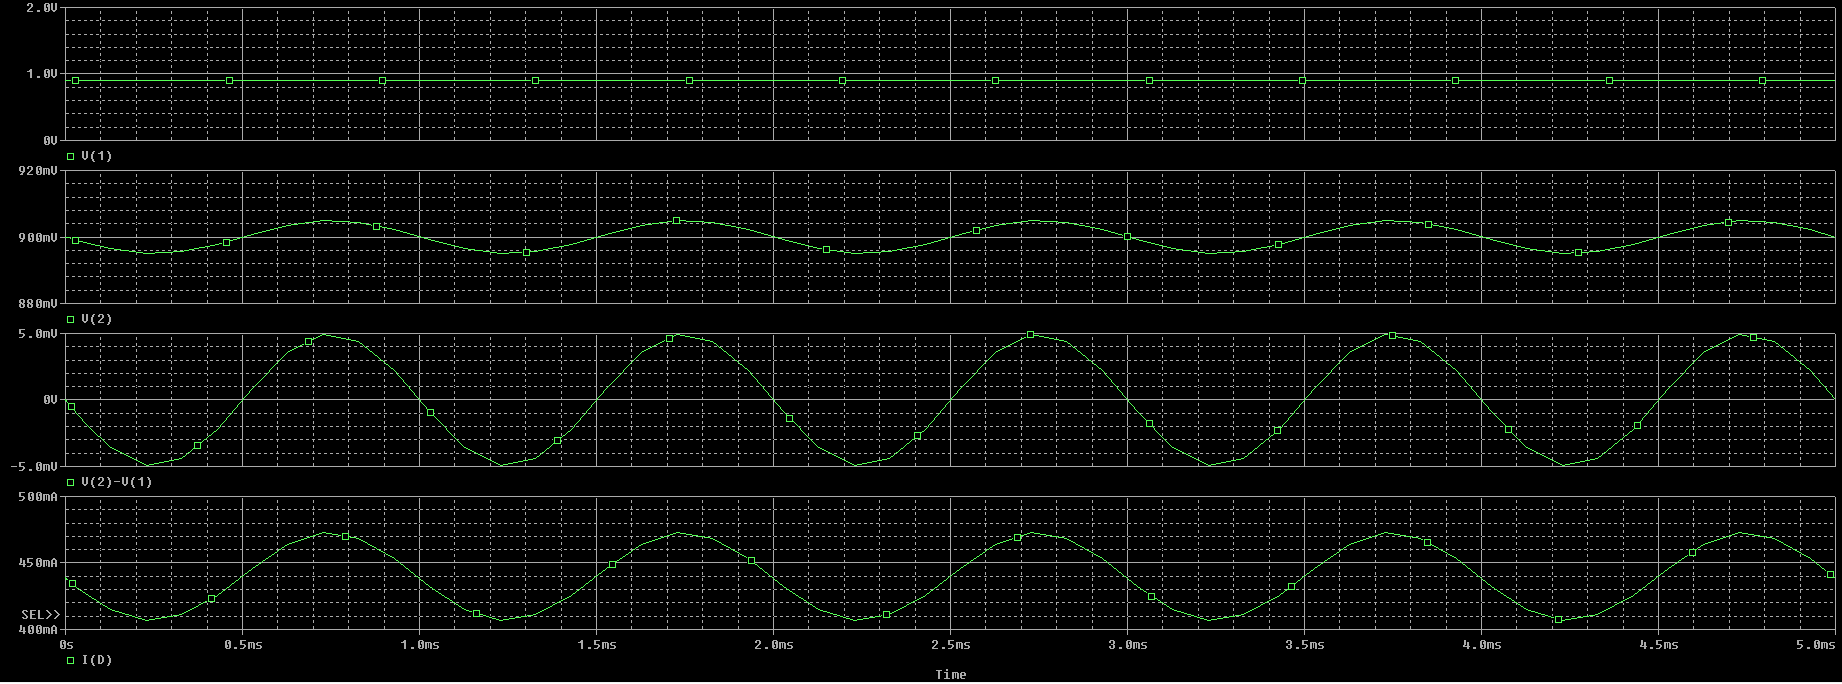
\includegraphics[width=\textwidth]{screenshots/Diode2.png}\\
    \textit{Visualisation de E, E(t), V(t), I(D)}\\
\end{center}

A partir des graphes V(t) et i(t), on déduit la résistance apparente. Pour cela, nous prenons un point sur chacun des graphes à l'instant \textbf{t}: \\

\begin{center}
    $R = \frac{V(t)}{I(t)} = \frac{0.9}{0.44} \approx 2\Omega$\\    
\end{center}

La valeur n'est pas conforme : $2\Omega \neq 0.1\Omega$\\


L'influence de l'amplitude est bloquant/passant. Losque \textit{V(2)} passe en dessous de la tension de seuil on  observe que la diode ce bloque. Cela explique l'anomalie sur le graphique ci-dessous:

\begin{center}
    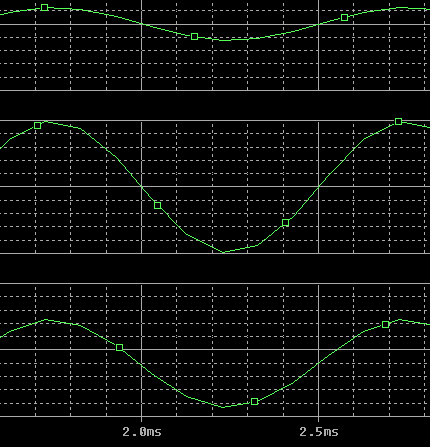
\includegraphics[width=0.5\textwidth]{screenshots/Diode3.png}\\
    \textit{Influence de l'amplitude - Centre de l'image}\\
\end{center}

L'influence de la fréquence est que la diode n'a pas le temps de commuté à l'instant du dépassement de seuil et prend du retard sur la commutation.\\

On le voit avec: \\

\begin{minted}[
    baselinestretch=1.4,
    bgcolor=LightGray,
    fontsize=\footnotesize]
{php}
DM
* DM3
.lib eval.lib
VE 1 0 DC=0.9
Vet 1 2 SIN (0 5m 70k 0 0 0)
D 2 0 D1N4002 ; diode de redressement
.TRAN 1u 100u
.probe
.end
\end{minted}

\begin{center}
    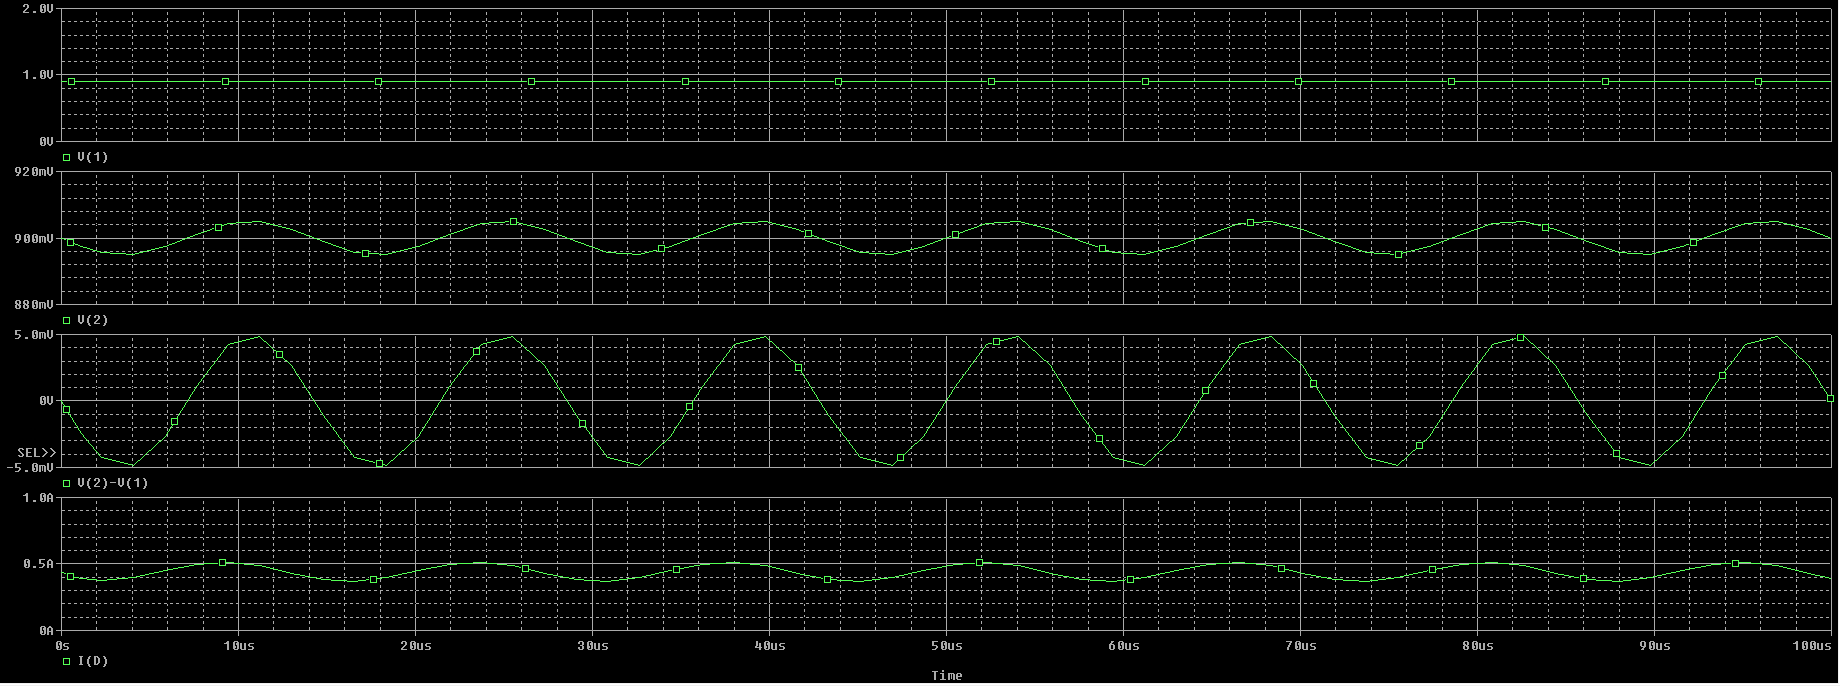
\includegraphics[width=\textwidth]{screenshots/Diode4.png}\\
    \textit{Influence de la fréquence - Déphasage}
\end{center}










\end{document}

\begin{minted}[
    baselinestretch=1.4,
    bgcolor=LightGray,
    fontsize=\footnotesize]
{php}

\end{minted}